\documentclass[a4paper, 11pt]{article}
\usepackage[T1]{fontenc}
\usepackage[utf8]{inputenc}
\usepackage[english]{babel}
\usepackage{mathtools}
\usepackage{amsfonts}
\usepackage{amsmath}
\usepackage{amsthm}
\usepackage{mathrsfs}
\usepackage{enumitem}
\usepackage{booktabs}
\usepackage{array}
\usepackage[skip=5pt, font=footnotesize]{caption}
% Useful floor and ceiling functions
\DeclarePairedDelimiter{\floor}{\lfloor}{\rfloor}
\DeclarePairedDelimiter{\ceil}{\lceil}{\rceil}
% Argmax/Argmin notation
\DeclareMathOperator*{\argmax}{argmax} 
\DeclareMathOperator*{\argmin}{argmin}
\DeclareMathOperator*{\rep}{rep} 
% Modified margins
%\usepackage[margin=2cm]{geometry}
% This avoids hypenation
\hyphenpenalty=1000
\usepackage{tikz}
\usetikzlibrary{arrows,calc,positioning,shadows,shapes}
\usepackage{graphicx}
\usepackage{subfig}
\graphicspath{{./images/}}
\captionsetup[figure]{labelfont={bf},name={Figure},labelsep=period}
\captionsetup[table]{labelfont={bf},name={Table},labelsep=period}

\usepackage{float}
\usepackage{xfrac}
\usepackage{pgfplots}
\usepackage{titling}
\usepackage[bottom]{footmisc}

\begin{document}

\begin{titlepage}

%\addtolength{\voffset}{-1.3cm}	

\vspace*{1cm}

\begin{center}
\large \textsc{Università degli Studi di Padova \\ Department of Information Engineering}

\vspace*{1cm}

\rule{\linewidth}{1pt} \Huge{ \textsc{Digital Forensics}} \\ {\textsc{Second Laboratory Report}} \rule{\linewidth}{2pt}

\vspace*{1cm}

\large \textsc{Faccin Dario} \\
\normalsize \textsc{ID Number: 1177736}

\end{center}

\section*{Abstract}
Digital visual media represent nowadays one of the principal means for communication. Lately, the reliability of digital visual information has been questioned, due to the ease in counterfeiting both its origin and content.

Digital image forensics is a research field which aims at validating the authenticity of images by recovering information about their history.

The main problem addressed in this report is the identification of the
imaging device that captured the image.
\end{titlepage}

\section*{Source identification}
\subsection*{Image acquisition process}
The light enters the imaging device through a system of optical lenses, which conveys it towards the imaging sensor. The imaging sensor is the heart of every digital camera, and it is composed of an array of photo detectors, each corresponding to a pixel of the final image, which transform the incoming light intensity into a proportional voltage.

Most cameras use CCD (Charged Coupled Device) sensors, but CMOS (Complementary Metal Oxide Semiconductor) imagers can also be found. To render color, before reaching the sensor the light is filtered by the Color Filter Array (CFA), a specific color mosaic that permits to each pixel to gather only one particular light wavelength (i.e. color). 

The CFA pattern arrangement depends on the manufacturer, although Bayer’s filter mosaic is often preferred. As a result, the sensor output is a mosaic of e.g. red, green and blue pixels arranged on a single layer.

To obtain the canonical 3-channels representation, the signal needs to be interpolated. Demosaicing algorithms are applied to this purpose; the missing pixel values in each layer are estimated based on the values of existing neighbors. Before the eventual storage, additional processing is performed, such as white balance, gamma correction, and image enhancement.

Finally, the image is recorded in the memory device. The following Figure \ref{fig:imacq} illustrates schematically the image acquisition process.

\begin{figure}[H]
	\centering
	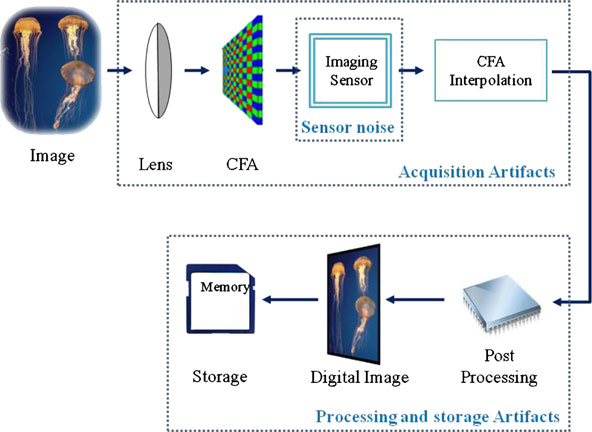
\includegraphics[width=0.5\textwidth]{imageacq}
	\caption{Image acquisition pipeline.}
	\label{fig:imacq}
\end{figure}

\subsection*{Camera identification}
The described image acquisition pipeline is common for most of the commercially
available devices. Each step is performed according to specific manufacturer
choices and hence might depend on the camera brand and model.

This variation can be used to determine the type of camera from which a specific image was obtained. Indeed, each stage in the pipeline can introduce imperfections in the final image or characteristic traits: lens distortion, chromatic aberration, pixel defects or CCD sensor imperfections, statistical dependencies related to proprietary CFA interpolation algorithms and other intrinsic image regularities.

These artifacts are statistically stable and can be considered as a signature of the camera type or even of the individual
device.

\section*{Sensor imperfections}
Imaging sensors have been shown to introduce various defects and to create noise in the
pixel values. The sensor noise is the result of three main components, i.e. pixel defects, \textit{Fixed Pattern Noise} (FPN), and \textit{Photo Response Non Uniformity} (PRNU).

Pixel defects include point defects, hot point defects, dead pixels, pixel traps, and cluster defects, which reasonably vary across different sensors, independent on the specific camera model.

FPN and PNRU are the two components of the so-called pattern noise, and depend on
dark currents in the sensor and pixel non-uniformities, respectively. Hence, they are
independent on the image content but closely related to the physical characteristics of each single sensor.

The pattern noise extracted from images taken by the same camera are more correlated than those extracted from different cameras.

\subsection*{Photo Response Non Uniformity}
Photo Response Non Uniformity (PRNU) is caused by the different sensitivity of the sensors to the light. This behavior is due to the manufacturing process and does not depend on the external temperature or acquisition time.

The resulting image can be described as following:
\begin{equation}
\mathbf{I} = \mathbf{I}^{(0)} + \mathbf{I}^{(0)} \mathbf{K} + \mathbf{\Theta}
\end{equation}
where $\mathbf{I}^{(0)}$ is the ideal sensor output (without noise), $\mathbf{K}$ is the PRNU fingerprint of the camera and $\mathbf{\Theta}$ accounts for all the other types of noise.

Pattern noise can be estimated by taking the difference between an image $\mathbf{I}$ and its denoised version:
\begin{equation}\label{eq:imdiff}
\mathbf{W_I} = \mathbf{I}- F\left(\mathbf{I}^{(0)}\right)
\end{equation}
where $\mathbf{W_I}$ is called \textit{residual noise} and $F$ is a \textit{denoising filter}.

\subsection*{PRNU fingerprint estimation}
Let $ \mathbf{\hat{I}}^{(0)}$ be the denoised version of $\mathbf{I}^{(0)}$.\\
We can rewrite Equation (\ref{eq:imdiff}) as:
\begin{align}
\mathbf{W_I} & = \mathbf{I}- \mathbf{\hat{I}}^{(0)} \nonumber \\
& = \mathbf{I}- \mathbf{\hat{I}}^{(0)} + \mathbf{I} \mathbf{K} - \mathbf{I} \mathbf{K} \nonumber \\
& = \mathbf{I} \mathbf{K} + \mathbf{I}^{(0)} - \mathbf{\hat{I}}^{(0)} + \left( \mathbf{I}^{(0)}-\mathbf{I} \right) \mathbf{K} + \mathbf{\Theta}
\end{align}
Now let $\mathbf{\Sigma} = \mathbf{I}^{(0)} - \mathbf{\hat{I}}^{(0)} + \left( \mathbf{I}^{(0)}-\mathbf{I} \right) \mathbf{K} + \mathbf{\Theta}$ be the noise independent from $\mathbf{IK}$. We can finally write:
\begin{equation}
\mathbf{W_I} = \mathbf{I} \mathbf{K} + \mathbf{\Sigma}
\end{equation}
Due to the random components related a specific image, the reference PNRU factor $\mathbf{\hat{K}}$ for a particular camera C is obtained can be estimated through Maximum Likelihood.

Given $N$ images $\mathbf{I}_1, \dots, \mathbf{I}_N$, we can reasonably assume that $\mathbf{\Sigma}[i]_1, \dots, \mathbf{\Sigma}[i]_N$ for each pixel $i$ are white Gaussian noise with variance $\sigma^2$. The energy of the PRNU $\mathbf{I} \mathbf{K}$ is small compared to the noise term $\Theta$, so we can also assume that $\mathbf{\Sigma}$ is independent of $\mathbf{I} \mathbf{K}$.\\
For each $i=1,\dots,N$ we have
\begin{equation*}
\dfrac{\mathbf{W}_i}{\mathbf{I}_i} = \mathbf{K} + \dfrac{\mathbf{\Sigma}_i}{\mathbf{I}_k}
\end{equation*}
The log-likelihood of observing $\dfrac{\mathbf{W}_i}{\mathbf{I}_i}$ given $\mathbf{K}$ is
\begin{equation}
L(\mathbf{K}) =-\dfrac{N}{2} \sum_{i=1}^{N}\log\left( \dfrac{2\pi\sigma^{2}}{({\bf I}_{i})^{2}}\right)-\sum_{i=1}^{N}{ \frac{\left(\dfrac{{\bf W}_{i}}{{\mathbf I}_{i}-{\bf K}}\right)^{2}}{\dfrac{2\sigma^{2}}{({\mathbf I}_{i})^{2}}}}
\end{equation}
The estimate is then obtained by computing the first order derivate of $L(\mathbf{K})$ with respect to $\mathbf{K}$ and solving for $\mathbf{K}$:
\begin{equation*}
\dfrac{\partial L(\mathbf{K})}{\partial{\bf K}} = 0 \implies \mathbf{\hat{K}} = \dfrac{\sum\limits_{i=1}^{N} \mathbf{W}_i \mathbf{I}_i}{\sum\limits_{i=1}^{N} \left( \mathbf{I}_i \right) ^2}
\end{equation*}
Computing the second order derivative is useful to obtain the Cramer-Rao lower bound and to infer what are the best images for the PRNU estimation.

\begin{equation}
\dfrac{ \partial^2 L(\mathbf{K})}{\partial \mathbf{K}^2} = \dfrac{\sigma^2}{\sum\limits_{i=1}^{N} \left( \mathbf{I}_i \right) ^2}
\end{equation}

The luminance $\mathbf{I}_i$ should be as high as possible but not saturated, since saturated pixels carry no information on the PRNU factor.

Also $\text{var}(\mathbf{\hat{K}}) \sim \sigma^2$, therefore better estimates are obtained using smooth test images.

\subsection*{PRNU fingerprint detection}

The estimated factor $\mathbf{\hat{K}}$ contains all components that are systematically present in every image. The most important are some weak artifacts of color interpolation, onsensor signal transfer and sensor design.

Such artifacts are not unique to the sensor and are shared among cameras of the same brand or cameras sharing the same imaging sensor design. The PRNU factors estimated from two different cameras may thus be slightly correlated, which would increase the false identification rate and decrease the reliability of camera identification.

To suppress these periodic traces in $\mathbf{\hat{K}}$, the mean of the rows and columns of the fingerprint is set to zero, and Wiener filtering is applied in the frequency domain after the maximum likelihood estimation.

These post operations increase the uniqueness of the fingerprint estimate among the same camera brand or model class.

This similarity of the estimated PRNU fingerprint can be measured by normalized cross correlation between $\mathbf{W_J}$ and $\mathbf{\hat{K}J}$ as:
\begin{equation}
\rho = corr \left( \mathbf{W_J}, \mathbf{\hat{K}J} \right)
\end{equation}
If the image $\mathbf{I_J}$ is not taken by camera X, the maximum of the correlation ratio $\max\{\rho\}$ is expected to be close to zero. If the image $\mathbf{I_J}$ is taken by camera X, then the correlation should be significantly higher than zero.

However, it is not possible to set a reliable detection threshold for all camera devices because of the different resolutions and sensor types.

This issue has been solved using a \textit{Peak-to-Correlation Energy} (PCE) ratio:
\begin{equation}
\text{PCE} = \dfrac{{\rho}^2_{\text{peak}}}{\frac{1}{|s|-|\epsilon|} \sum\limits_{s\notin \epsilon} {\rho}^2_s}
\end{equation}
where ${\rho}_{\text{peak}}$ is the supremum of the normalized cross correlation between $\mathbf{W_J}$ and $\mathbf{\hat{K}J}$ and $s$ is the map to all entries of $\rho$. $\epsilon$ represents a small, centered region around ${\rho}_{\text{peak}}$, whereas $|s|-|\epsilon|$ is the total number of entries outside $\epsilon$.

\section*{Results}
The \textsc{Matlab} code provided for this assignment performs the PRNU estimation and detection.

Among the returned values, the most important are the \textit{Peak-to-Correlation Energy} (PCE) and the \textit{Probability of False Alarm} (P\_FA).

One tunable parameter is \texttt{windowsize}: this parameter allows the user to choose the span, in pixels, to consider for both the PRNU estimation and then detection.

For the data set provided with the code we have 6 flat-field images on which we estimate the PRNU fingerprint and 11 images whose origin is to predict.

Before running the script, we analyzed the EXIF information stored in both the flat-field and natural images. The flat-field images are taken by a \textit{LG V30 (H930)}, while the natural images are taken by five different devices: \textit{OnePlus 6T (A6013)}, \textit{OnePlus 5 (A5000)}, \textit{LG V30 (H930)}, \textit{OnePlus 6 (A6003)}, \textit{Xiaomi Mi A2 Lite}.

The following Table \ref{tab:defaultdataset} shows the results of the code running on the provided data set:
\begin{table}[H]
	\centering

	\begin{tabular}{c|c|c|c|c|c}
	Image & Acquisition Device & PCE (512) & PCE (2048) & $P_{FA}$ (512) & $P_{FA}$ (2048) \\
	\hline
	\texttt{nat\_01} & OnePlus 6T (A6013)	& 6.0638	& -1.0006 & 0.0069 & 0.8414 \\
	\texttt{nat\_02} & OnePlus 5 (A5000) 	& 0.0892	& 0.1314 & 0.3826 & 0.8535 \\
	\texttt{nat\_03} & LG V30 (H930) 	& 37.2846	& 681.8796	& 5.1044e-10 & 1.3036e-150\\
	\texttt{nat\_04} & OnePlus 6 (A6003) 	& -0.1512	& 3.0514	& 0.6513 & 0.0403 \\
	\texttt{nat\_05} & LG V30 (H930) 		& 46.7558	& 993.4452 & 4.0203e-12 & 2.3880e-218\\
	\texttt{nat\_06} & LG V30 (H930) 	& 124.5864	& 1.3225e+03 & 3.1345e-29 & 7.2932e-290\\
	\texttt{nat\_07} & Xiaomi Mi A2 Lite	& -4.8861	& -0.5088 & 0.9865 & 0.7622 \\
	\texttt{nat\_08} & Xiaomi Mi A2 Lite 	& 0.0036	& 2.2319 & 0.4760 & 0.0676 \\
	\texttt{nat\_09} & OnePlus 6T (A6013)	& -0.2413	& -0.0808 & 0.6884 & 0.6119\\
	\texttt{nat\_10} & OnePlus 6 (A6003) 	& 0.0132	& 0.0023 & 0.4542 & 0.4808\\
	\texttt{nat\_11} & LG V30 (H930) 		& 26.7829	& 156.8201 & 1.1382e-07 & 2.8018e-36
	\end{tabular}
	\caption{Results obtained for the default data set, for two parameters \texttt{windowsize}.}
	\label{tab:defaultdataset}
\end{table}

From Table \ref{tab:defaultdataset} we see that the images associated with an ``high'' PCE value and ``low'' probability of false alarm are the ones which are taken by the same device used for the PRNU fingerprint estimation.

Increasing the tunable parameter \texttt{windowsize} did improve the accuracy in the detection: while in the first case (512 pixels) one image (\texttt{nat\_01}) has non-negligible PCE (6.0638), in the second case (2048 pixels) it is instead negligible (-1.0006). On the other hand the main drawback is the increased complexity and therefore processing processing time increases.

These results are more clear when looking at Figure \ref{fig:defaultdataset512} and Figure \ref{fig:defaultdataset2048}, which present the pair $(PCE,P_{FA})$ for each image, in both linear and logarithmic scale.

\begin{figure}[H]
	\centering
	\subfloat{
	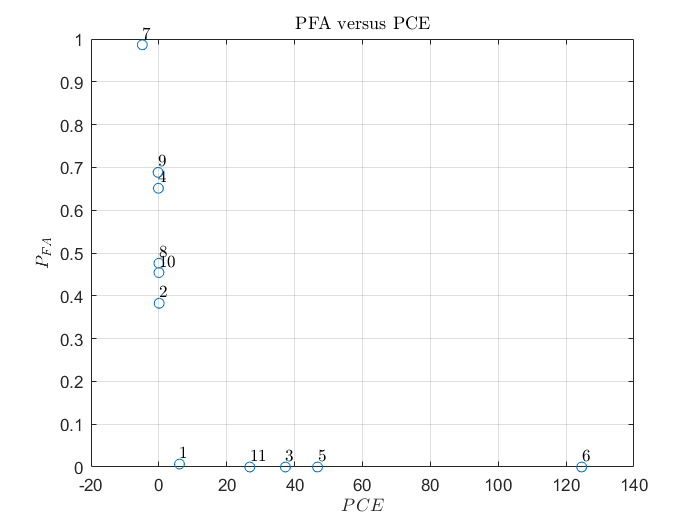
\includegraphics[width=0.4\textwidth]{defaultdataset512}}
	\subfloat{
	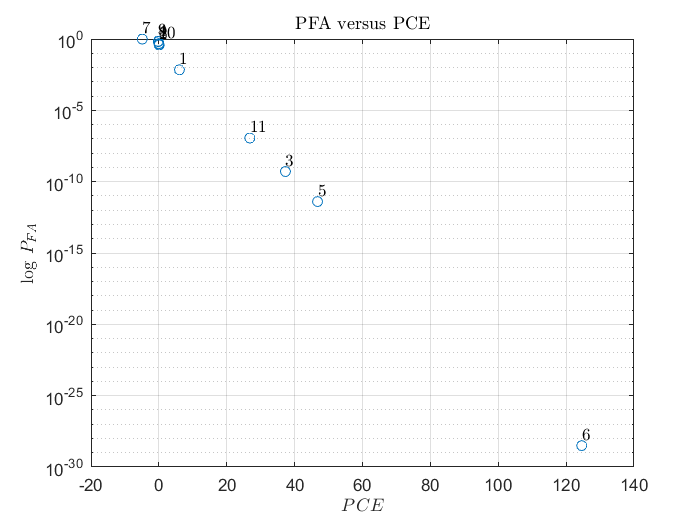
\includegraphics[width=0.4\textwidth]{defaultdataset512log}}
	\caption{Results obtained for the default data set, for \texttt{windowsize=512}.}
	\label{fig:defaultdataset512}
\end{figure}
\begin{figure}[H]
	\centering
	\subfloat{
	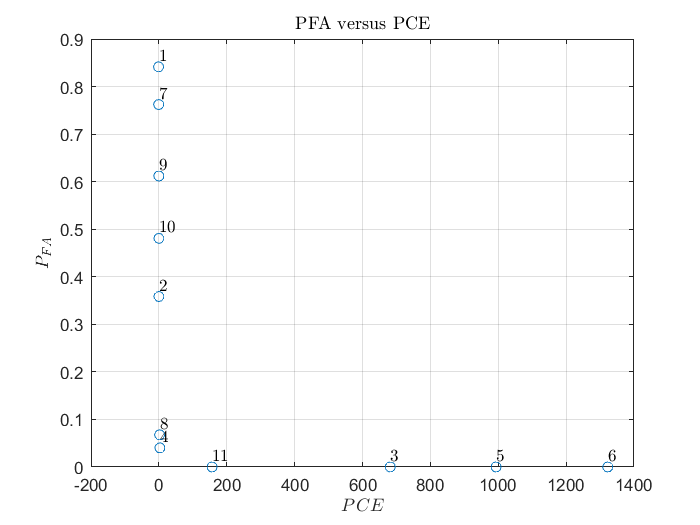
\includegraphics[width=0.4\textwidth]{defaultdataset2048}}
	\subfloat{
	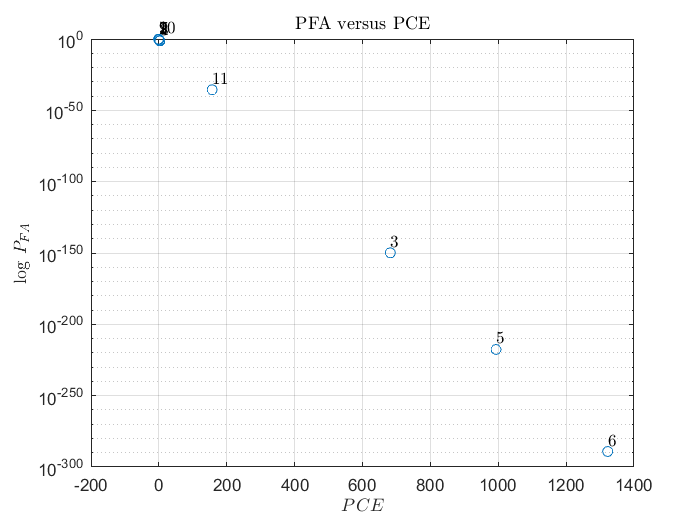
\includegraphics[width=0.4\textwidth]{defaultdataset2048log}}
	\caption{Results obtained for the default data set, for \texttt{windowsize=2048}.}
	\label{fig:defaultdataset2048}
\end{figure}

The previous analysis has then been repeated using flat-field images taken by a \textit{Canon EOS M50} and test images as before, plus two images from the incriminated camera.

\begin{table}[H]
	\centering	
	\begin{tabular}{c|c|c|c}
		Image			 & Acquisition Device	& PCE (512)	& $P_{FA}$ (512) \\
		\toprule
		\texttt{nat\_01} & OnePlus 6T (A6013)	& -0.1751	& 0.6622 \\
		\texttt{nat\_02} & OnePlus 5 (A5000) 	& 0.0236	& 0.4389 \\
		\texttt{nat\_03} & LG V30 (H930) 		& -3.0625	& 0.9599 \\
		\texttt{nat\_04} & OnePlus 6 (A6003) 	& -0.8005	& 0.8145 \\
		\texttt{nat\_05} & LG V30 (H930) 		& 1.8642	& 0.0861 \\
		\texttt{nat\_06} & LG V30 (H930) 		& -0.0491	& 0.5876 \\
		\texttt{nat\_07} & Xiaomi Mi A2 Lite	& -0.0687	& 0.6033 \\
		\texttt{nat\_08} & Xiaomi Mi A2 Lite 	& 4.6016	& 0.0160 \\
		\texttt{nat\_09} & OnePlus 6T (A6013)	& 2.0962 	& 0.0738 \\
		\texttt{nat\_10} & OnePlus 6 (A6003) 	& 1.5389	& 0.1074 \\
		\texttt{nat\_11} & LG V30 (H930) 		& 0.1089	& 0.3707 \\
		\texttt{nat\_13} & Canon EOS M50		& 400.2607	& 2.4163e-89 \\
		\texttt{nat\_13} & Canon EOS M50		& 828.0930	& 2.1049e-182
	\end{tabular}
	\caption{Results obtained for the modified data set, for \texttt{windowsize=512}.}
	\label{tab:modifieddataset}
\end{table}

From Figure \ref{fig:modifieddataset512} it is possible to see graphically how better the algorithm performs in this situation, despite the low value for \texttt{windowsize} (512 pixels).

\begin{figure}[H]
	\centering
	\subfloat{
		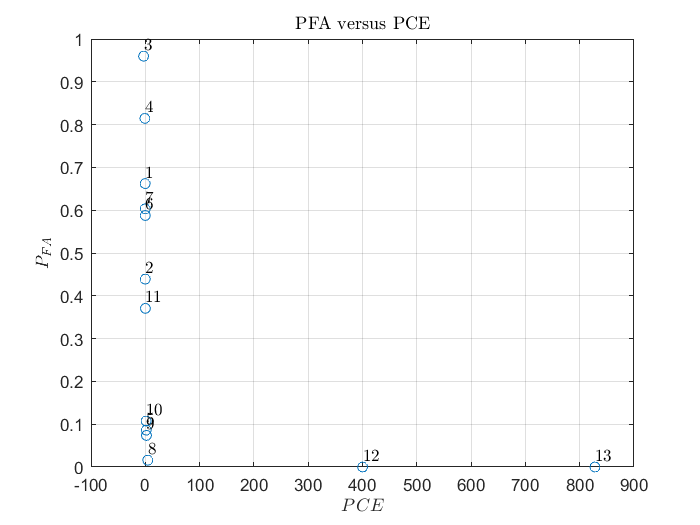
\includegraphics[width=0.4\textwidth]{modifieddataset512}}
	\subfloat{
		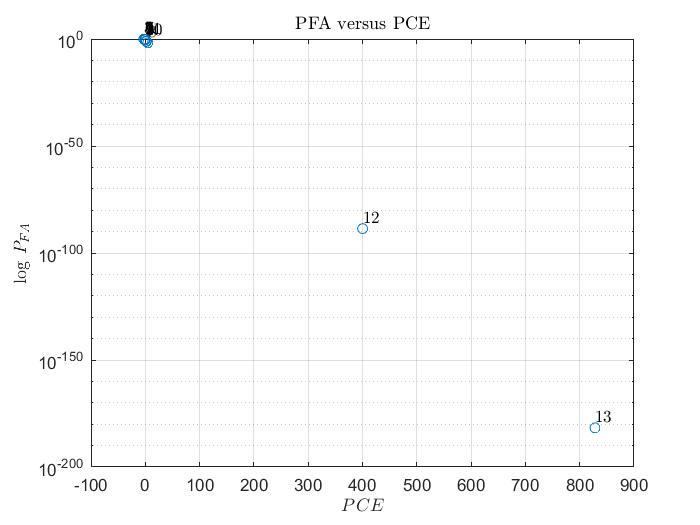
\includegraphics[width=0.4\textwidth]{modifieddataset512log}}
	\caption{Results obtained for the modified data set, for \texttt{windowsize=1024}.}
	\label{fig:modifieddataset512}
\end{figure}

The following Figure \ref{fig:timerequired} shows how the parameter \texttt{windowsize} affects the computational time of the PRNU estimation and detection:
\begin{figure}[H]
	\centering
	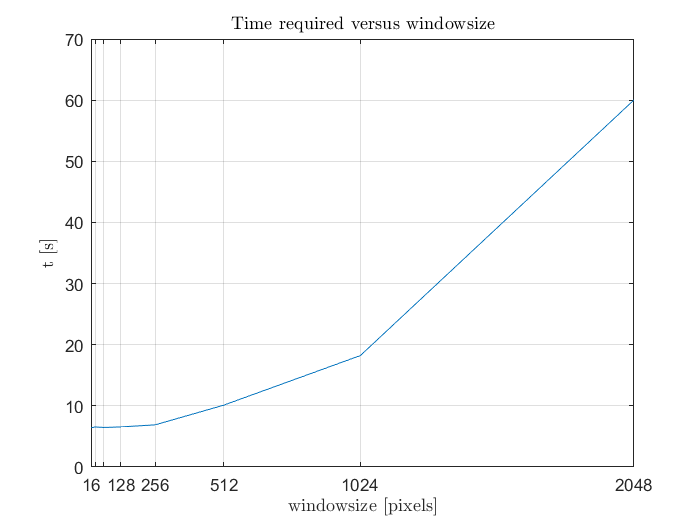
\includegraphics[width=0.4\textwidth]{timerequired}
	\caption{Time required for different \texttt{windowsize}.}
	\label{fig:timerequired}
\end{figure}

Regarding the algorithm complexity, the \textit{Curve Fitting Toolbox} provided by \textsc{Matlab} has been used to roughly estimate whether the behavior is exponential or no.

The following Figure \ref{fig:curvefitting} shows how the software interpolated the data we have:
\begin{figure}[H]
	\centering
	\subfloat[Full fitting.]{
		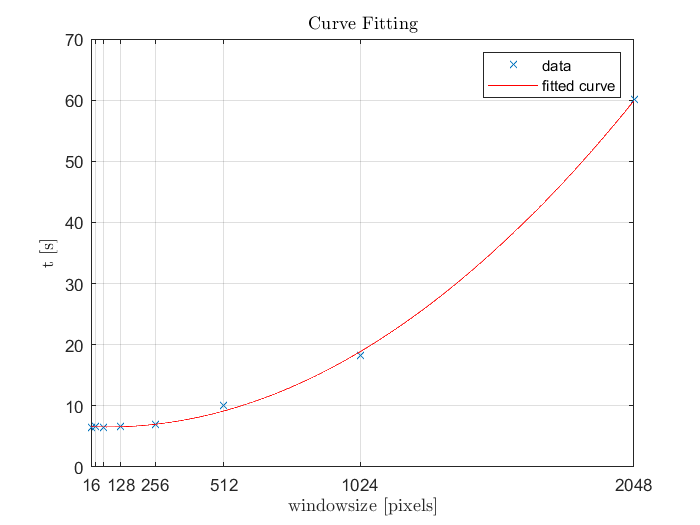
\includegraphics[width=0.4\textwidth]{curvefitting}}
	\subfloat[Zoom.]{
		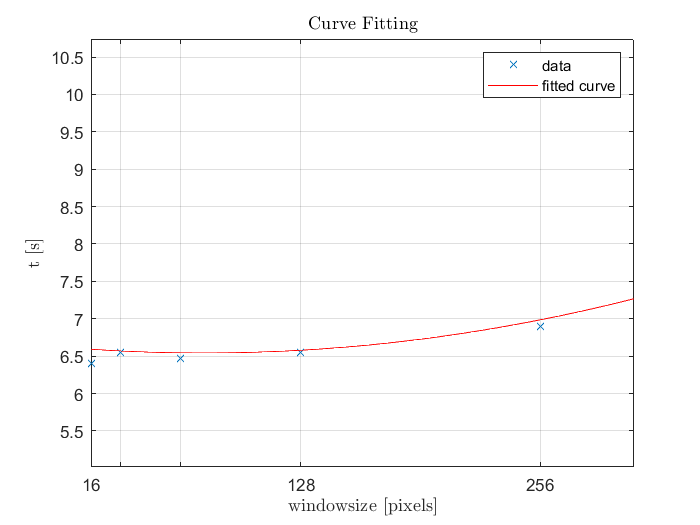
\includegraphics[width=0.4\textwidth]{curvefittingzoomed}}
	\caption{Results of the fitting.}
	\label{fig:curvefitting}
\end{figure}

The algorithm complexity can be modeled both as quadratic or exponential function:
\begin{equation}
C_{PRNU}(x) = \left( 1.373\cdot 10^{-5} \right) x^2 + 6.622
\end{equation}
\begin{equation}
C_{PRNU}(x) = 5.701 e^{0.00115 x}
\end{equation}
where $x$ is the \texttt{windowsize}.\\

Now we evaluate the detection performance using the one single image but with different compression ratios.

Despite the original image being already compressed in a lossy form (JPEG standard), for the sake of the analysis we consider it as uncompressed. Therefore we would expect better performance if the original image is in an uncompressed format (RAW).

What we expect is that the PRNU detection works linearly with the quality of the image, meaning that as the image quality decreases the detection would degrade.

In Figure \ref{fig:differentquality} the test image (\texttt{nat\_05}) versions are numbered in increasing order of compression ratio (1: original ``uncompressed'' image, 13: most compressed). 

\begin{figure}[H]
	\centering
	\subfloat[Results in linear scale.]{
		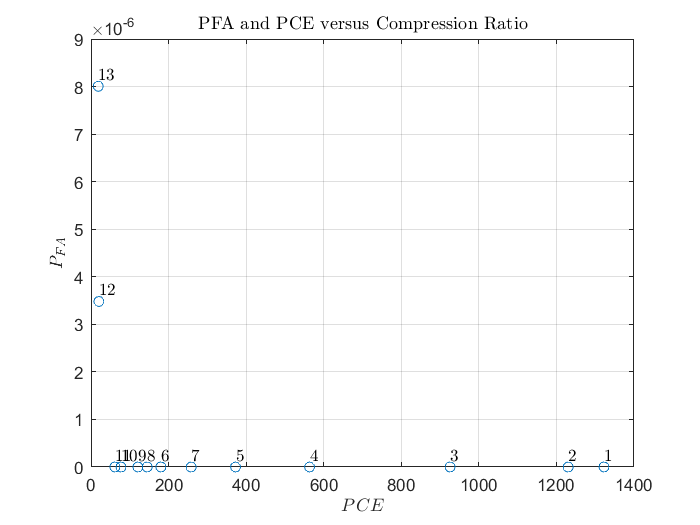
\includegraphics[width=0.5\textwidth]{testcr}}
	\subfloat[Results in logarithmic scale.]{
		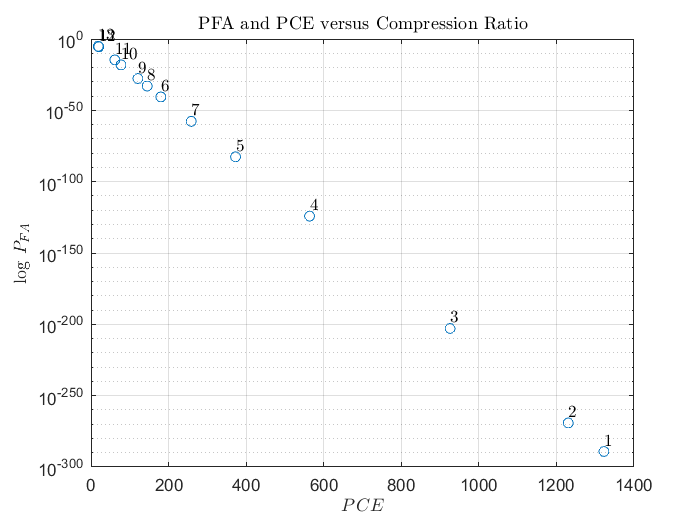
\includegraphics[width=0.5\textwidth]{testcrlog}}
	\caption{Results obtained for image \texttt{nat\_05}.}
	\label{fig:differentquality}
\end{figure}

\begin{thebibliography}{3}
	\bibitem{paper1}
	Chen M., Fridrich J., Goljan M., Lukáš J.,
	\textit{Determining Image Origin and Integrity Using Sensor Noise}.
	2008.
	
	\bibitem{paper2}
	Dirik A. E., Karaküçük A.,
	\textit{Forensic use of photo response non-uniformity of imaging sensors and a counter method}.
	2014.
		
	\bibitem{dig}
	Dugelay J., Redi J., Taktak W.,
	\textit{Digital image forensics}.
	2010.
	
	\bibitem{digitalf}
	Milani S.,
	\textit{Digital Forensics: course lectures}.
	2018.
\end{thebibliography}

\end{document}